\section{Zielsetzung}

In diesem Versuch werden Relaxationsphänomene am Beispiel eines $RC$-Kreises näher betrachtet. Hierbei wird die Relaxationszeitkonstante des $RC$-Kreises einmal
über die Betrachtung eines Ent- oder Aufladevorgangs eines Kondensators über einen Widerstand, einmal durch die Veränderung der Amplitude bei hohen Frequenzen 
und einmal durch die auftretende Phasenverschiebung zwischen Kondensator- und Speisespannung bei hohen Frequenzen ermittelt.
\section{Theorie}
\label{sec:Theorie}

\subsection{Allgemeine Relaxationsgleichung}

    Relaxationsphänomene treten auf, wenn ein System aus seinem Ausgangszustand herausgenommen wird und sich diesem nicht-ozsillatorisch wieder annähert.
    Wird die physikalische Größe A betrachtet, gilt:
    \begin{equation} \label{eq:relaxation}
        \frac{\symup{d}A}{\symup{d}t}=c[A(t)-A(\infty)]
    \end{equation}
    Daraus folgt 
    \begin{equation*}
        \int_{A(0)}^{A(t)} \frac{\symup{d}A'}{A' - A(\infty)} = \int_0^t c \,\symup{d}t' \implies \text{ln} \frac{A(t) - A(\infty)}{A(0) - A(\infty)} = ct,
    \end{equation*}
    sodass sich als Funktion schließlich
    \begin{equation*}
        A(t) = A(\infty) + [A(0) - A(\infty)] \text{e}^{ct}
    \end{equation*}
    ergibt. Hier muss $c<0$ gelten, da $A$ sonst nicht beschränkt sein würde. Die Relaxationszeitkonstante ist durch den Ausduck $\sfrac{1}{c}$ gegeben.


\subsection{Entlade- und Aufladevorgang eines RC-Kreises}

    Ein RC-Kreis ist ein Schaltkreis bestehend aus einem Widerstand R und einem Kondensator mit der Kapazität C. Sein Auf- und Entladevorgang ist ein gutes Beispiel 
    für auftretende Relaxationsvorgänge. In der \autoref{fig:Auf_Entladen} ist ein Schaltkreis zu sehen, welcher zum Auf- und Entladen eines Kondensators über einen 
    Widerstand geeignet ist.

    \begin{figure}[H]
        \centering
        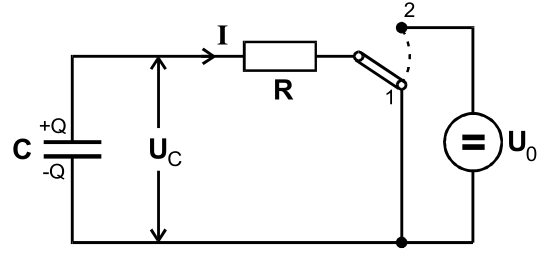
\includegraphics[width=0.6\textwidth]{bilder/Auflade_und_entlade.PNG}
        \caption{Der Schaltkreis zum Aufladen (2) und Entladen (1) eines Kondensators über einen Widerstand.\cite{anleitung}}
        \label{fig:Auf_Entladen}
    \end{figure}

    \noindent
    Unter der Annahme, dass sich auf den Platten des Kondensators der Kapazität $C$ die Ladung $Q$ befindet, lässt sich eine Spannung 
    \begin{equation*}
        U_{\text{C}} = \frac{Q}{C}
    \end{equation*}
    messen. Für diese gilt nach dem Ohm'schen Gesetz $I = \frac{U_{\text{C}}}{R}$ und der Relation $\frac{\symup{d}Q}{\symup{d}t} = -I$:
    \begin{equation*}
        \frac{\symup{d}Q}{\symup{d}t}  = - \frac{1}{RC} Q(t)
    \end{equation*}
    Diese Gleichung zeigt große Ähnlichkeit zu der allgemeinen Relaxationsgleichung \eqref{eq:relaxation} auf. Es gilt $Q(\infty) = 0$, da der Kondensator nach 
    unendlicher Zeit vollständig entladen ist. Somit kann für den Entladevorgang direkt gefolgert werden:
    \begin{equation}
        \label{eqn:AufgabeA}
        Q(t) = Q(0) \text{exp}(-t/RC)
    \end{equation}
    Analog kann für den Aufladevorgang die Gleichung
    \begin{equation*}
        Q(t) = CU_0(1- \text{exp}(-t/RC))
    \end{equation*}
    hergeleitet werden, wobei die Speisespannung mit $U_0$ bezeichnet wird und für die Ladung $Q(0)= 0 $ und $Q(\infty) = CU_0 $ gilt.
    Die Zeitkonstante des Relaxationsvorganges ist in diesem Fall gegeben durch $RC$. Sie gibt den Zeitraum an, in dem sich hier die Ladung auf dem Kondensator 
    um den Faktor $\sfrac{1}{\symup{e}}$ verändert.

\subsection{Relaxation bei periodischer Auslenkung aus Gleichgewichtslage}

    Auch im weiteren wird der RC-Kreis betrachtet, wobei in dem Schaltkreis in \autoref{fig:per_ausl} das Vorgehen klarer hervorgeht. Es ist zu erwarten, dass es bei
    einer Speisespannung der Form $U(t) = U_0 \cos(\omega t)$ mit steigender Frequenz zu einer Amplitudenabnahme und Phasenverschiebung der Kondensatorspannung 
    kommt.

    \begin{figure}[H]
        \centering
        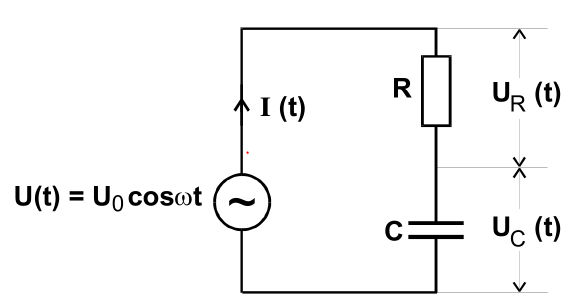
\includegraphics[width=0.6\textwidth]{bilder/periodische_Auslenkung.PNG}
        \caption{Ein Schaltkreis mit einer Reihenschaltung eines Kondensator und eines Widerstandes gespeist von einer sinus-förmigen Spannung. \cite{anleitung}}
        \label{fig:per_ausl}
    \end{figure}

    \noindent Für die Kondensatorspannung $U_{\text{C}}$ wird folgender Ansatz gemacht:
    \begin{equation*}
        U_{\text{C}} = A (\omega) \cdot \cos( \omega t + \varphi(\omega) )
    \end{equation*}
    Werden die Realtionen $U_{\text{R}} = I \cdot R $ (Ohm'sches Gesetz) und $I = \frac{\symup{d}Q}{\symup{d}t} = C \cdot \frac{\symup{d}U_{\text{C}}}{\symup{d}t}$
    in das zweite Kirchhof'sche Gesetz (Maschenregel) 
    \begin{equation*}
        U(t) = U_{\text{R}} + U_{\text{C}}
    \end{equation*}
    eingesetzt, so folgt die Gleichung:
    \begin{equation}\label{eqn:kirchhoff_eingesetzt}
        U_0 \cos(\omega t) = -A \omega R C \sin(\omega t + \varphi) + A(\omega) \cos(\omega t + \varphi)
    \end{equation}
    Da diese Gleichung für alle $t$ gelten muss, wird $\omega t = \frac{\pi}{2} $ gesetzt. Nun werden $\sin(\frac{\pi}{2} + \varphi) = \cos(\varphi)$ und 
    $\cos(\frac{\pi}{2} + \varphi) = -\sin(\varphi)$ genutzt. Somit ergibt sich für die Gleichung \eqref{eqn:kirchhoff_eingesetzt}:
    \begin{equation*}
        0 = - \omega RC \cos(\varphi) - \sin(\varphi)
    \end{equation*}
    Für die Phasenverschiebung lässt sich nun die Abhängigkeit 
    \begin{equation} \label{eqn:phasenverschiebung}
        \varphi(\omega) = \arctan(-\omega R C)
    \end{equation}
    herleiten. Anhand der Gleichung \eqref{eqn:phasenverschiebung} ist zu erkennen, dass für eine kleine Frequenz $f$, welche im Zusammenhang $\omega = 2\pi f$ mit 
    der Kreisfreqenz $\omega$ steht, die Phasenverschiebung $\varphi$ sehr gering ist und für sehr hohe Frequenzen die Grenzphasenverschiebung von 
    $\varphi = \frac{\pi}{2}$ angenähert wird. Trifft die Kreisfrequenz genau $\omega = \frac{1}{RC}$, so ergibt sich eine Phasenverschiebung von $\varphi = \frac{\pi}{4}$.


    \noindent Um einen Ausdruck für die Veränderung der Amplitude zu bekommen, wird der Ausdruck $\omega t + \varphi = \frac{\pi}{2}$ gesetzt und in die Gleichung
    \eqref{eqn:kirchhoff_eingesetzt} eingesetzt. Dies ist möglich, da die Gleichung \eqref{eqn:kirchhoff_eingesetzt} für alle Werte von $t$ gelten muss.
    Es ergibt sich:
    \begin{equation}
        \label{eqn:AufgabeD}
        U_0 \cos(\frac{\pi}{2} - \varphi) = -A \omega RC  \iff A(\omega) = - \frac{\sin(\varphi)}{\omega RC }U_0
    \end{equation}
    Mithilfe des trigonometrischen Pythagoras lässt sich aus der Formel \eqref{eqn:phasenverschiebung} 
    \begin{equation*}
        \sin(\varphi) = \frac{\omega RC}{\sqrt{1 + \omega^2 R^2 C^2}}
    \end{equation*}
    herleiten. Somit lautet der Ausdruck zur Veränderung der Amplitude:
    \begin{equation} \label{eqn:amplitude}
        A(\omega) = \frac{U_0}{\sqrt{1 + \omega^2 R^2 C^2}}
    \end{equation}
    Es ist auffällig, dass kleine Frequenzen die Amplitude recht klein und unverändert lassen, während für sehr hohe Frequenzen die Amplitude gegen Null geht. 
    Daher werden solche $RC$-Kreise als Tiefpässe eingesetzt, wobei hier kritisiert wird, dass die Amplitude nur mit $\frac{1}{ \omega}$ gegen Null geht.


\subsection{RC-Kreis als Integrator}

    Es ist möglich, dass eine zeitlich veränderliche angelegte Spannung in einem $RC$-Kreis integriert wird. Mithilfe des Kirchhoff'schen Gesetz, dem Ohm'schen 
    Gesetz und der Relation $\frac{\symup{d}Q}{\symup{d}t} = I$ , kann folgende Formel aufgestellt werden:
    \begin{equation*}
        U(t) = U_{\text{R}}(t) + U_{\text{C}}(t) = I(t)R + U_{\text{C}}(t) = RC \cdot \frac{\symup{d}U_{\text{C}}}{\symup{d}t} + U_{\text{C}} 
    \end{equation*}
    Mit den Ahnnahmen, dass $\omega \gg \frac{1}{RC}$, $|U_{\text{C}}| \ll |U_{\text{R}}|$ und $|U_{\text{C}}| \ll |U| $ gilt:
    \begin{equation*}
        U(t) = RC \frac{\symup{d}U_{\text{C}}}{\symup{d}t}
    \end{equation*}
    Somit ist das Integral 
    \begin{equation*}
        U_{\text{C}} (t) = \frac{1}{RC} \int_0^{t'} U(t') \, \symup{d}t'
    \end{equation*}
    berechenbar. 